\newpage
\begin{landscape}
\section{Project Tasks and Schedule}
\begin{figure}[H]
\centering
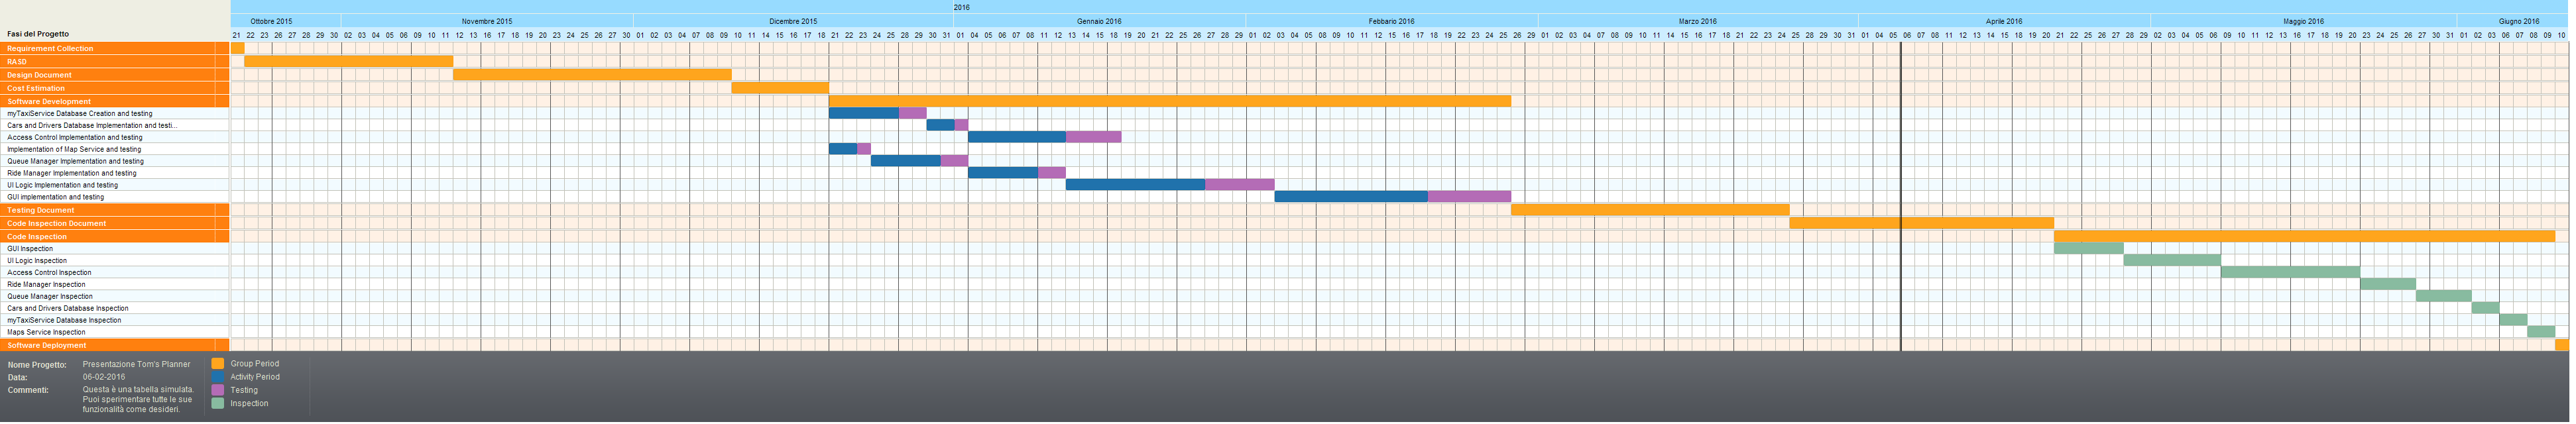
\includegraphics[scale=0.25]{DiagramSources/Ganttingsoftware2.png}
\label{Figure 1: }\caption{Gantt diagram of the project}
\end{figure}
\end{landscape}
In this section is presented the Gantt diagram of our project.\\
On 21\textsuperscript{st} October it has been set the meeting with the company that required us to project myTaxiService application. During this day we talked about features and goals of the software to develop. We estimated the collection of this information requires only one day to be completed. \\
From the 22\textsuperscript{nd} of October to the 11\textsuperscript{th} of November we worked on RASD: using information gather during the meeting, we prepared the document to present it before the deadline. \\
Following Gantt diagram, it is possible to see that we continued our project writing the DD and like the previous document, we guaranteed the applicants to complete it in more or less a month. \\
After these two documents, we thought it was the time to write the Project Plan document, keeping one month the time necessary to conclude and to present it. \\
Software development is the next task, we estimate this phase will last approximately two months taking into consideration code writing part and the testing one. \\
Composition of Testing document is the next step and it will last four weeks. It will contains all mistakes present in developed code. \\
We continue with Code Inspection document that will show how various components have to test each other. Two months are necessary to complete inspection phase. \\
At the end, we will deploy the software to the company on 10\textsuperscript{th} June. \\
The overall time requested to complete the project is eight months as we estimated. \\
As you can see from Gantt diagram, weekends are not considered working day (due to working laws).\\      